\chapter{Construction de volumes englobants}%boîtes englobantes orientées}
\label{app:obb}

L'objet de cette annexe est de proposer des méthodes pour la construction de volumes englobants des courbes et surfaces paramétriques polynomiales exprimées dans les bases de Chebyshev ou Bernstein.
On se limite à des boîtes (parallélépipèdes rectangles) dont l'orientation dans l'espace est déterminée à l'aide d'heuristiques simples. Un bon compromis est ainsi trouvé entre l'étroitesse des boîtes et la complexité de leur construction, qui est proportionnelle au degré de la paramétrisation polynomiale.
%cf. notes ``Intersections''\par\medskip
%L'objet de cette annexe est de donner une heuristique pour la construction de volumes englobants compacts pour des courbes et surfaces paramétriques polynomiales exprimées dans les bases de Chebyshev ou Bernstein.
%On se limite à des boîtes (parallélépipèdes rectangles) dont l'orientation dans l'espace est choisie à l'aide d'une heuristique simple, qui offre un bon compromis entre 
%On se limite à des boîtes (parallélépipèdes rectangles) d'orientation arbitraire, qui semblent représenter un bon compromis entre les complexités de construction et de détection de collisions.
%La complexité de leur construction croit linéairement avec le degré de la paramétrisation polynomiale, et englobent étroitement
%Un compromis doit être trouvé entre, d'une part la complexité de construction de 
%On choisit d'utiliser des boîtes (parallélépipèdes rectangles) orientées de façon à trouver un compromis entre, d'une part la complexité de construction


\section{Définition}
On définit une boîte orientée de centre $\vrm{c}$, de demi-côtés $\family{a}{i}{1}{3}$ et d'axes (orthonormés) $\family{\vrm{e}}{i}{1}{3}$ comme l'ensemble des points $\bx \in \mathbb{R}^3$ qui vérifient, pour $i=1,2,3$,
\begin{equation}
	\left| \dotprod{\vrm{e}_i}{\left(\bx - \vrm{c}\right)} \right| \leq a_i.
	\label{eq:def_obb}
\end{equation}

\begin{figure}
\centering
%\includegraphics[width=8cm]{figures/code/obb-1.mps}
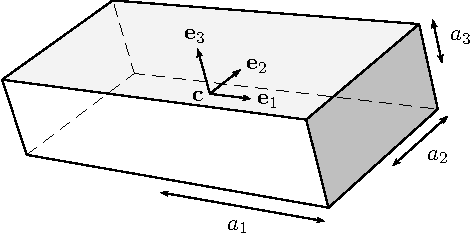
\includegraphics[scale=1]{figures/obb.pdf}
%\chapter{Construction de volumes englobants}%boîtes englobantes orientées}
\label{app:obb}

L'objet de cette annexe est de proposer des méthodes pour la construction de volumes englobants des courbes et surfaces paramétriques polynomiales exprimées dans les bases de Chebyshev ou Bernstein.
On se limite à des boîtes (parallélépipèdes rectangles) dont l'orientation dans l'espace est déterminée à l'aide d'heuristiques simples. Un bon compromis est ainsi trouvé entre l'étroitesse des boîtes et la complexité de leur construction, qui est proportionnelle au degré de la paramétrisation polynomiale.
%cf. notes ``Intersections''\par\medskip
%L'objet de cette annexe est de donner une heuristique pour la construction de volumes englobants compacts pour des courbes et surfaces paramétriques polynomiales exprimées dans les bases de Chebyshev ou Bernstein.
%On se limite à des boîtes (parallélépipèdes rectangles) dont l'orientation dans l'espace est choisie à l'aide d'une heuristique simple, qui offre un bon compromis entre 
%On se limite à des boîtes (parallélépipèdes rectangles) d'orientation arbitraire, qui semblent représenter un bon compromis entre les complexités de construction et de détection de collisions.
%La complexité de leur construction croit linéairement avec le degré de la paramétrisation polynomiale, et englobent étroitement
%Un compromis doit être trouvé entre, d'une part la complexité de construction de 
%On choisit d'utiliser des boîtes (parallélépipèdes rectangles) orientées de façon à trouver un compromis entre, d'une part la complexité de construction


\section{Définition}
On définit une boîte orientée de centre $\vrm{c}$, de demi-côtés $\family{a}{i}{1}{3}$ et d'axes orthonormés $\family{\vrm{e}}{i}{1}{3}$ comme l'ensemble des points $\bx \in \mathbb{R}^3$ qui vérifient, pour $i=1,2,3$,
\begin{equation}
	\left| \dotprod{\vrm{e}_i}{\left(\bx - \vrm{c}\right)} \right| \leq a_i.
	\label{eq:def_obb}
\end{equation}

\begin{figure}
\centering
%\includegraphics[width=8cm]{figures/code/obb-1.mps}
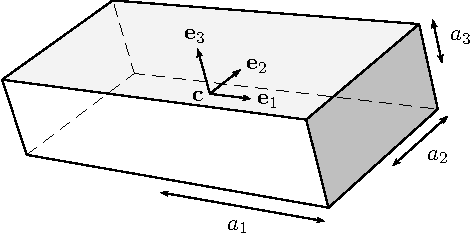
\includegraphics[scale=1]{figures/obb.pdf}
%\chapter{Construction de volumes englobants}%boîtes englobantes orientées}
\label{app:obb}

L'objet de cette annexe est de proposer des méthodes pour la construction de volumes englobants des courbes et surfaces paramétriques polynomiales exprimées dans les bases de Chebyshev ou Bernstein.
On se limite à des boîtes (parallélépipèdes rectangles) dont l'orientation dans l'espace est déterminée à l'aide d'heuristiques simples. Un bon compromis est ainsi trouvé entre l'étroitesse des boîtes et la complexité de leur construction, qui est proportionnelle au degré de la paramétrisation polynomiale.
%cf. notes ``Intersections''\par\medskip
%L'objet de cette annexe est de donner une heuristique pour la construction de volumes englobants compacts pour des courbes et surfaces paramétriques polynomiales exprimées dans les bases de Chebyshev ou Bernstein.
%On se limite à des boîtes (parallélépipèdes rectangles) dont l'orientation dans l'espace est choisie à l'aide d'une heuristique simple, qui offre un bon compromis entre 
%On se limite à des boîtes (parallélépipèdes rectangles) d'orientation arbitraire, qui semblent représenter un bon compromis entre les complexités de construction et de détection de collisions.
%La complexité de leur construction croit linéairement avec le degré de la paramétrisation polynomiale, et englobent étroitement
%Un compromis doit être trouvé entre, d'une part la complexité de construction de 
%On choisit d'utiliser des boîtes (parallélépipèdes rectangles) orientées de façon à trouver un compromis entre, d'une part la complexité de construction


\section{Définition}
On définit une boîte orientée de centre $\vrm{c}$, de demi-côtés $\family{a}{i}{1}{3}$ et d'axes orthonormés $\family{\vrm{e}}{i}{1}{3}$ comme l'ensemble des points $\bx \in \mathbb{R}^3$ qui vérifient, pour $i=1,2,3$,
\begin{equation}
	\left| \dotprod{\vrm{e}_i}{\left(\bx - \vrm{c}\right)} \right| \leq a_i.
	\label{eq:def_obb}
\end{equation}

\begin{figure}
\centering
%\includegraphics[width=8cm]{figures/code/obb-1.mps}
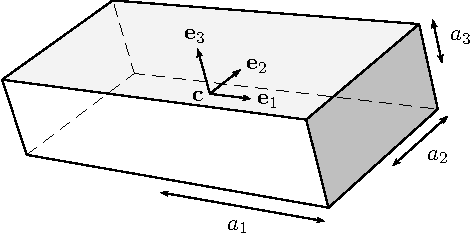
\includegraphics[scale=1]{figures/obb.pdf}
%\chapter{Construction de volumes englobants}%boîtes englobantes orientées}
\label{app:obb}

L'objet de cette annexe est de proposer des méthodes pour la construction de volumes englobants des courbes et surfaces paramétriques polynomiales exprimées dans les bases de Chebyshev ou Bernstein.
On se limite à des boîtes (parallélépipèdes rectangles) dont l'orientation dans l'espace est déterminée à l'aide d'heuristiques simples. Un bon compromis est ainsi trouvé entre l'étroitesse des boîtes et la complexité de leur construction, qui est proportionnelle au degré de la paramétrisation polynomiale.
%cf. notes ``Intersections''\par\medskip
%L'objet de cette annexe est de donner une heuristique pour la construction de volumes englobants compacts pour des courbes et surfaces paramétriques polynomiales exprimées dans les bases de Chebyshev ou Bernstein.
%On se limite à des boîtes (parallélépipèdes rectangles) dont l'orientation dans l'espace est choisie à l'aide d'une heuristique simple, qui offre un bon compromis entre 
%On se limite à des boîtes (parallélépipèdes rectangles) d'orientation arbitraire, qui semblent représenter un bon compromis entre les complexités de construction et de détection de collisions.
%La complexité de leur construction croit linéairement avec le degré de la paramétrisation polynomiale, et englobent étroitement
%Un compromis doit être trouvé entre, d'une part la complexité de construction de 
%On choisit d'utiliser des boîtes (parallélépipèdes rectangles) orientées de façon à trouver un compromis entre, d'une part la complexité de construction


\section{Définition}
On définit une boîte orientée de centre $\vrm{c}$, de demi-côtés $\family{a}{i}{1}{3}$ et d'axes orthonormés $\family{\vrm{e}}{i}{1}{3}$ comme l'ensemble des points $\bx \in \mathbb{R}^3$ qui vérifient, pour $i=1,2,3$,
\begin{equation}
	\left| \dotprod{\vrm{e}_i}{\left(\bx - \vrm{c}\right)} \right| \leq a_i.
	\label{eq:def_obb}
\end{equation}

\begin{figure}
\centering
%\includegraphics[width=8cm]{figures/code/obb-1.mps}
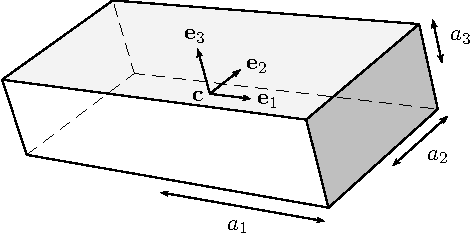
\includegraphics[scale=1]{figures/obb.pdf}
%\input{figures/obb.tex}
\caption{Boîte orientée.}
\end{figure}

%Une telle boîte est un polyèdre convexe, on peut donc appliquer le \textit{théorème des axes séparateurs} afin de déterminer si l’intersection de deux boîtes orientées est vide ou non \cite{eberly2002}.
   
\section{Base de Chebyshev}
Les méthodes présentées dans cette section reposent sur une propriété fondamentale des polynômes de Chebyshev : pour tout $n \in \mathbb{N}$ et pour tout $-1 \leq x \leq 1$,
\begin{equation}
	\left| T_n(x) \right| \leq 1.
\end{equation}

\subsection{Boîte englobant une courbe}
Soit $\Gamma$ un segment de courbe décrit par la paramétrisation 
\begin{align}
  \bg \colon \chebinterval &\longrightarrow \Gamma \subset \mathbb{R}^3 \nonumber \\
  t\; &\longmapsto \sum_{n=0}^{N} \hat{\bg}_n T_n(t).
\end{align}
%
La série tronquée
\begin{equation}
	\truncseries{\bg}{1}(t) = \sum_{n=0}^{1} \hat{\bg}_n T_n(t)
\end{equation}
définit une bonne approximation linéaire de $\Gamma$, à savoir la droite passant par le point $\hat{\bg}_0$ et dirigée par le vecteur $\hat{\bg}_1$. 
%\par
On choisit donc $\vrm{c} = \hat{\bg}_0$ comme centre de la boîte, et on définit le premier axe comme
\begin{equation}
	\vrm{e}_1 = \unitized{\hat{\bg}_1}.
\end{equation}
On construit ensuite les axes $\vrm{e}_2$ et $\vrm{e}_3$ en suivant le procédé d'orthonormalisation de Gram-Schmidt. Si $\normtwo{\hat{\bg}_1} \ll 1$, on construit une boîte alignée avec les axes du repère cartésien.
\par
%On calcule ensuite les demi-côtés de la boîte. 
Pour $-1 \leq t \leq 1$ et $i=1,2,3$,
\begin{align*}
	\dotprod{\vrm{e}_i}{\left( \bg(t) - \vrm{c} \right)} 
	&= \dotprod{\vrm{e}_i}{\sum_{n=1}^{N} \hat{\bg}_n T_n(t)} ,\\
	&= \sum_{n=1}^{N}\dotprod{\vrm{e}_i}{\hat{\bg}_n} T_n(t),
\end{align*}
donc
\begin{equation*}
	\left| \dotprod{\vrm{e}_i}{\left( \bg(t) - \vrm{c} \right)} \right| 
	\leq \sum_{n=1}^{N} \left|\dotprod{\vrm{e}_i}{\hat{\bg}_n}\right| \left| T_n(t) \right|.
\end{equation*}
Or, pour tous $n \in \mathbb{N}$ et $t \in \chebinterval$, $\left| T_n(t) \right| \leq 1$, 
%\begin{align*}
%	\left| \dotprod{\vrm{e}_i}{\left( \bg(t) - \vrm{c} \right)} \right| 
%	\leq& \sum_{n=1}^{N} \left|\dotprod{\vrm{e}_i}{\hat{\bg}_n}\right| \left| T_n(t) \right|,\\
%	\leq& \sum_{n=1}^{N} \left|\dotprod{\vrm{e}_i}{\hat{\bg}_n}\right|.
%\end{align*}
donc en choisissant
\begin{equation}
	a_i = \sum_{n=1}^{N} \left|\dotprod{\vrm{e}_i}{\hat{\bg}_n}\right|,
\end{equation}
la boîte orientée contient bien $\Gamma$.


\subsection{Boîte englobant une surface}
Soit $\Sigma$ un carreau de surface décrit par la paramétrisation 
\begin{align}
  \bs \colon \chebinterval^2 &\longrightarrow \Sigma \subset \mathbb{R}^3 \nonumber \\
  (u,v)\; &\longmapsto \sum_{m=0}^{M} \sum_{n=0}^{N} \hat{\bs}_{m,n} T_m(u) T_n(v).
\end{align}
%
%La série tronquée
%\begin{equation}
%	\truncseries{\bs}{1}(u,v) = 
%	\hat{\bs}_{0,0} T_0(u) T_0(v) + 
%	\hat{\bs}_{1,0} T_1(u) T_0(v) +
%	\hat{\bs}_{0,1} T_0(u) T_1(v)
%\end{equation}
%définit une bonne approximation linéaire de $\Sigma$, à savoir le plan passant par le point $\hat{\bs}_{0,0}$ et engendré par les vecteur $\hat{\bs}_{1,0}$ et $\hat{\bs}_{0,1}$.
Sans restreindre la généralité, on suppose que $\normtwo{\hat{\bs}_{1,0}} \geq \normtwo{\hat{\bs}_{0,1}}$.
\par
Le plan passant par le point $\hat{\bs}_{0,0}$ et engendré par les vecteurs $\hat{\bs}_{1,0}$ et $\hat{\bs}_{0,1}$ est une bonne approximation linéaire de $\Sigma$. 
%\par
On choisit donc $\vrm{c} = \hat{\bs}_{0,0}$ comme centre de la boîte, et on définit le premier axe comme
\begin{equation}
	\vrm{e}_1 = \unitized{\hat{\bs}_{1,0}}.
\end{equation}
On définit les troisième et deuxième axes comme 
\begin{equation}
	\vrm{e}_3 = \unitized{\crossprod{\hat{\bs}_{1,0}}{\hat{\bs}_{0,1}}},
\end{equation}
et
\begin{equation}
	\vrm{e}_2 = \crossprod{\vrm{e}_3}{\vrm{e}_1}.
\end{equation}
Si $\normtwo{\crossprod{\hat{\bs}_{1,0}}{\hat{\bs}_{0,1}}} \ll 1$, on construit une boîte alignée avec les axes du repère cartésien.
%surface potentiellement dégénérée en une courbe suivant un des deux paramètres u ou v, cf boite englobante de courbe, sinon AABB
\par
Pour $-1 \leq u, v \leq 1$,
%\begin{align*}
%	\dotprod{\vrm{e}_i}{\left( \bs(u,v) - \vrm{c} \right)} 
%	&= \dotprod{\vrm{e}_i}{%
%	\sum_{m=1}^{M} \hat{\bs}_{m,0} T_m(u) +
%	\sum_{n=1}^{N} \hat{\bs}_{0,n} T_n(v) + 
%	\sum_{m=1}^{M} \sum_{n=1}^{N} \hat{\bs}_{m,n} T_m(u) T_n(v)
%	}
%\end{align*}
\begin{equation}
	\bs(u,v) - \vrm{c} =
	\sum_{m=1}^{M} \hat{\bs}_{m,0} T_m(u) +
	\sum_{n=1}^{N} \hat{\bs}_{0,n} T_n(v) + 
	\sum_{m=1}^{M} \sum_{n=1}^{N} \hat{\bs}_{m,n} T_m(u) T_n(v).
\end{equation}
Donc, pour $i = 1,2,3$,
%\begin{equation}
%	\left| \dotprod{\vrm{e}_i}{\left( \bs(u,v) - \vrm{c} \right)} \right| 
%	\leq
%	\sum_{m=1}^{M} \left| \dotprod{\vrm{e}_i}{\hat{\bs}_{m,0}} \right| + 
%	\sum_{n=1}^{N} \left| \dotprod{\vrm{e}_i}{\hat{\bs}_{0,n}} \right| + 
%	\sum_{m=1}^{M} \sum_{n=1}^{N} \left| \dotprod{\vrm{e}_i}{\hat{\bs}_{m,n}} \right|.
%\end{equation}
\begin{align}
	\left| \dotprod{\vrm{e}_i}{\left( \bs(u,v) - \vrm{c} \right)} \right| \leq &
	\sum_{m=1}^{M} \left| \dotprod{\vrm{e}_i}{\hat{\bs}_{m,0}} \right| \left| T_m(u) \right| + 
	\sum_{n=1}^{N} \left| \dotprod{\vrm{e}_i}{\hat{\bs}_{0,n}} \right| \left| T_n(v) \right| \nonumber \\
	&+ \sum_{m=1}^{M} \sum_{n=1}^{N} \left| \dotprod{\vrm{e}_i}{\hat{\bs}_{m,n}} \right| \left| T_m(u) \right| \left| T_n(v) \right| ,\nonumber \\
	\leq &
	\sum_{m=1}^{M} \left| \dotprod{\vrm{e}_i}{\hat{\bs}_{m,0}} \right| + 
	\sum_{n=1}^{N} \left| \dotprod{\vrm{e}_i}{\hat{\bs}_{0,n}} \right| + 
	\sum_{m=1}^{M} \sum_{n=1}^{N} \left| \dotprod{\vrm{e}_i}{\hat{\bs}_{m,n}} \right|.
\end{align}
En choisissant
\begin{equation}
	a_i = 
	\sum_{m=0}^{M} \sum_{n=0}^{N} \left| \dotprod{\vrm{e}_i}{\hat{\bs}_{m,n}} \right|
	- \left| \dotprod{\vrm{e}_i}{\hat{\bs}_{0,0}} \right|, 
\end{equation}
la boîte orientée contient bien $\Sigma$.
%
%
%
\section{Base de Bernstein}
%Les polynômes de Bernstein $\family{B^{N}}{n}{0}{N}$ forment une partition de l'unité sur $\berninterval$.


\caption{Boîte orientée.}
\end{figure}

%Une telle boîte est un polyèdre convexe, on peut donc appliquer le \textit{théorème des axes séparateurs} afin de déterminer si l’intersection de deux boîtes orientées est vide ou non \cite{eberly2002}.
   
\section{Base de Chebyshev}
Les méthodes présentées dans cette section reposent sur une propriété fondamentale des polynômes de Chebyshev : pour tout $n \in \mathbb{N}$ et pour tout $-1 \leq x \leq 1$,
\begin{equation}
	\left| T_n(x) \right| \leq 1.
\end{equation}

\subsection{Boîte englobant une courbe}
Soit $\Gamma$ un segment de courbe décrit par la paramétrisation 
\begin{align}
  \bg \colon \chebinterval &\longrightarrow \Gamma \subset \mathbb{R}^3 \nonumber \\
  t\; &\longmapsto \sum_{n=0}^{N} \hat{\bg}_n T_n(t).
\end{align}
%
La série tronquée
\begin{equation}
	\truncseries{\bg}{1}(t) = \sum_{n=0}^{1} \hat{\bg}_n T_n(t)
\end{equation}
définit une bonne approximation linéaire de $\Gamma$, à savoir la droite passant par le point $\hat{\bg}_0$ et dirigée par le vecteur $\hat{\bg}_1$. 
%\par
On choisit donc $\vrm{c} = \hat{\bg}_0$ comme centre de la boîte, et on définit le premier axe comme
\begin{equation}
	\vrm{e}_1 = \unitized{\hat{\bg}_1}.
\end{equation}
On construit ensuite les axes $\vrm{e}_2$ et $\vrm{e}_3$ en suivant le procédé d'orthonormalisation de Gram-Schmidt. Si $\normtwo{\hat{\bg}_1} \ll 1$, on construit une boîte alignée avec les axes du repère cartésien.
\par
%On calcule ensuite les demi-côtés de la boîte. 
Pour $-1 \leq t \leq 1$ et $i=1,2,3$,
\begin{align*}
	\dotprod{\vrm{e}_i}{\left( \bg(t) - \vrm{c} \right)} 
	&= \dotprod{\vrm{e}_i}{\sum_{n=1}^{N} \hat{\bg}_n T_n(t)} ,\\
	&= \sum_{n=1}^{N}\dotprod{\vrm{e}_i}{\hat{\bg}_n} T_n(t),
\end{align*}
donc
\begin{equation*}
	\left| \dotprod{\vrm{e}_i}{\left( \bg(t) - \vrm{c} \right)} \right| 
	\leq \sum_{n=1}^{N} \left|\dotprod{\vrm{e}_i}{\hat{\bg}_n}\right| \left| T_n(t) \right|.
\end{equation*}
Or, pour tous $n \in \mathbb{N}$ et $t \in \chebinterval$, $\left| T_n(t) \right| \leq 1$, 
%\begin{align*}
%	\left| \dotprod{\vrm{e}_i}{\left( \bg(t) - \vrm{c} \right)} \right| 
%	\leq& \sum_{n=1}^{N} \left|\dotprod{\vrm{e}_i}{\hat{\bg}_n}\right| \left| T_n(t) \right|,\\
%	\leq& \sum_{n=1}^{N} \left|\dotprod{\vrm{e}_i}{\hat{\bg}_n}\right|.
%\end{align*}
donc en choisissant
\begin{equation}
	a_i = \sum_{n=1}^{N} \left|\dotprod{\vrm{e}_i}{\hat{\bg}_n}\right|,
\end{equation}
la boîte orientée contient bien $\Gamma$.


\subsection{Boîte englobant une surface}
Soit $\Sigma$ un carreau de surface décrit par la paramétrisation 
\begin{align}
  \bs \colon \chebinterval^2 &\longrightarrow \Sigma \subset \mathbb{R}^3 \nonumber \\
  (u,v)\; &\longmapsto \sum_{m=0}^{M} \sum_{n=0}^{N} \hat{\bs}_{m,n} T_m(u) T_n(v).
\end{align}
%
%La série tronquée
%\begin{equation}
%	\truncseries{\bs}{1}(u,v) = 
%	\hat{\bs}_{0,0} T_0(u) T_0(v) + 
%	\hat{\bs}_{1,0} T_1(u) T_0(v) +
%	\hat{\bs}_{0,1} T_0(u) T_1(v)
%\end{equation}
%définit une bonne approximation linéaire de $\Sigma$, à savoir le plan passant par le point $\hat{\bs}_{0,0}$ et engendré par les vecteur $\hat{\bs}_{1,0}$ et $\hat{\bs}_{0,1}$.
Sans restreindre la généralité, on suppose que $\normtwo{\hat{\bs}_{1,0}} \geq \normtwo{\hat{\bs}_{0,1}}$.
\par
Le plan passant par le point $\hat{\bs}_{0,0}$ et engendré par les vecteurs $\hat{\bs}_{1,0}$ et $\hat{\bs}_{0,1}$ est une bonne approximation linéaire de $\Sigma$. 
%\par
On choisit donc $\vrm{c} = \hat{\bs}_{0,0}$ comme centre de la boîte, et on définit le premier axe comme
\begin{equation}
	\vrm{e}_1 = \unitized{\hat{\bs}_{1,0}}.
\end{equation}
On définit les troisième et deuxième axes comme 
\begin{equation}
	\vrm{e}_3 = \unitized{\crossprod{\hat{\bs}_{1,0}}{\hat{\bs}_{0,1}}},
\end{equation}
et
\begin{equation}
	\vrm{e}_2 = \crossprod{\vrm{e}_3}{\vrm{e}_1}.
\end{equation}
Si $\normtwo{\crossprod{\hat{\bs}_{1,0}}{\hat{\bs}_{0,1}}} \ll 1$, on construit une boîte alignée avec les axes du repère cartésien.
%surface potentiellement dégénérée en une courbe suivant un des deux paramètres u ou v, cf boite englobante de courbe, sinon AABB
\par
Pour $-1 \leq u, v \leq 1$,
%\begin{align*}
%	\dotprod{\vrm{e}_i}{\left( \bs(u,v) - \vrm{c} \right)} 
%	&= \dotprod{\vrm{e}_i}{%
%	\sum_{m=1}^{M} \hat{\bs}_{m,0} T_m(u) +
%	\sum_{n=1}^{N} \hat{\bs}_{0,n} T_n(v) + 
%	\sum_{m=1}^{M} \sum_{n=1}^{N} \hat{\bs}_{m,n} T_m(u) T_n(v)
%	}
%\end{align*}
\begin{equation}
	\bs(u,v) - \vrm{c} =
	\sum_{m=1}^{M} \hat{\bs}_{m,0} T_m(u) +
	\sum_{n=1}^{N} \hat{\bs}_{0,n} T_n(v) + 
	\sum_{m=1}^{M} \sum_{n=1}^{N} \hat{\bs}_{m,n} T_m(u) T_n(v).
\end{equation}
Donc, pour $i = 1,2,3$,
%\begin{equation}
%	\left| \dotprod{\vrm{e}_i}{\left( \bs(u,v) - \vrm{c} \right)} \right| 
%	\leq
%	\sum_{m=1}^{M} \left| \dotprod{\vrm{e}_i}{\hat{\bs}_{m,0}} \right| + 
%	\sum_{n=1}^{N} \left| \dotprod{\vrm{e}_i}{\hat{\bs}_{0,n}} \right| + 
%	\sum_{m=1}^{M} \sum_{n=1}^{N} \left| \dotprod{\vrm{e}_i}{\hat{\bs}_{m,n}} \right|.
%\end{equation}
\begin{align}
	\left| \dotprod{\vrm{e}_i}{\left( \bs(u,v) - \vrm{c} \right)} \right| \leq &
	\sum_{m=1}^{M} \left| \dotprod{\vrm{e}_i}{\hat{\bs}_{m,0}} \right| \left| T_m(u) \right| + 
	\sum_{n=1}^{N} \left| \dotprod{\vrm{e}_i}{\hat{\bs}_{0,n}} \right| \left| T_n(v) \right| \nonumber \\
	&+ \sum_{m=1}^{M} \sum_{n=1}^{N} \left| \dotprod{\vrm{e}_i}{\hat{\bs}_{m,n}} \right| \left| T_m(u) \right| \left| T_n(v) \right| ,\nonumber \\
	\leq &
	\sum_{m=1}^{M} \left| \dotprod{\vrm{e}_i}{\hat{\bs}_{m,0}} \right| + 
	\sum_{n=1}^{N} \left| \dotprod{\vrm{e}_i}{\hat{\bs}_{0,n}} \right| + 
	\sum_{m=1}^{M} \sum_{n=1}^{N} \left| \dotprod{\vrm{e}_i}{\hat{\bs}_{m,n}} \right|.
\end{align}
En choisissant
\begin{equation}
	a_i = 
	\sum_{m=0}^{M} \sum_{n=0}^{N} \left| \dotprod{\vrm{e}_i}{\hat{\bs}_{m,n}} \right|
	- \left| \dotprod{\vrm{e}_i}{\hat{\bs}_{0,0}} \right|, 
\end{equation}
la boîte orientée contient bien $\Sigma$.
%
%
%
\section{Base de Bernstein}
%Les polynômes de Bernstein $\family{B^{N}}{n}{0}{N}$ forment une partition de l'unité sur $\berninterval$.


\caption{Boîte orientée.}
\end{figure}

%Une telle boîte est un polyèdre convexe, on peut donc appliquer le \textit{théorème des axes séparateurs} afin de déterminer si l’intersection de deux boîtes orientées est vide ou non \cite{eberly2002}.
   
\section{Base de Chebyshev}
Les méthodes présentées dans cette section reposent sur une propriété fondamentale des polynômes de Chebyshev : pour tout $n \in \mathbb{N}$ et pour tout $-1 \leq x \leq 1$,
\begin{equation}
	\left| T_n(x) \right| \leq 1.
\end{equation}

\subsection{Boîte englobant une courbe}
Soit $\Gamma$ un segment de courbe décrit par la paramétrisation 
\begin{align}
  \bg \colon \chebinterval &\longrightarrow \Gamma \subset \mathbb{R}^3 \nonumber \\
  t\; &\longmapsto \sum_{n=0}^{N} \hat{\bg}_n T_n(t).
\end{align}
%
La série tronquée
\begin{equation}
	\truncseries{\bg}{1}(t) = \sum_{n=0}^{1} \hat{\bg}_n T_n(t)
\end{equation}
définit une bonne approximation linéaire de $\Gamma$, à savoir la droite passant par le point $\hat{\bg}_0$ et dirigée par le vecteur $\hat{\bg}_1$. 
%\par
On choisit donc $\vrm{c} = \hat{\bg}_0$ comme centre de la boîte, et on définit le premier axe comme
\begin{equation}
	\vrm{e}_1 = \unitized{\hat{\bg}_1}.
\end{equation}
On construit ensuite les axes $\vrm{e}_2$ et $\vrm{e}_3$ en suivant le procédé d'orthonormalisation de Gram-Schmidt. Si $\normtwo{\hat{\bg}_1} \ll 1$, on construit une boîte alignée avec les axes du repère cartésien.
\par
%On calcule ensuite les demi-côtés de la boîte. 
Pour $-1 \leq t \leq 1$ et $i=1,2,3$,
\begin{align*}
	\dotprod{\vrm{e}_i}{\left( \bg(t) - \vrm{c} \right)} 
	&= \dotprod{\vrm{e}_i}{\sum_{n=1}^{N} \hat{\bg}_n T_n(t)} ,\\
	&= \sum_{n=1}^{N}\dotprod{\vrm{e}_i}{\hat{\bg}_n} T_n(t),
\end{align*}
donc
\begin{equation*}
	\left| \dotprod{\vrm{e}_i}{\left( \bg(t) - \vrm{c} \right)} \right| 
	\leq \sum_{n=1}^{N} \left|\dotprod{\vrm{e}_i}{\hat{\bg}_n}\right| \left| T_n(t) \right|.
\end{equation*}
Or, pour tous $n \in \mathbb{N}$ et $t \in \chebinterval$, $\left| T_n(t) \right| \leq 1$, 
%\begin{align*}
%	\left| \dotprod{\vrm{e}_i}{\left( \bg(t) - \vrm{c} \right)} \right| 
%	\leq& \sum_{n=1}^{N} \left|\dotprod{\vrm{e}_i}{\hat{\bg}_n}\right| \left| T_n(t) \right|,\\
%	\leq& \sum_{n=1}^{N} \left|\dotprod{\vrm{e}_i}{\hat{\bg}_n}\right|.
%\end{align*}
donc en choisissant
\begin{equation}
	a_i = \sum_{n=1}^{N} \left|\dotprod{\vrm{e}_i}{\hat{\bg}_n}\right|,
\end{equation}
la boîte orientée contient bien $\Gamma$.


\subsection{Boîte englobant une surface}
Soit $\Sigma$ un carreau de surface décrit par la paramétrisation 
\begin{align}
  \bs \colon \chebinterval^2 &\longrightarrow \Sigma \subset \mathbb{R}^3 \nonumber \\
  (u,v)\; &\longmapsto \sum_{m=0}^{M} \sum_{n=0}^{N} \hat{\bs}_{m,n} T_m(u) T_n(v).
\end{align}
%
%La série tronquée
%\begin{equation}
%	\truncseries{\bs}{1}(u,v) = 
%	\hat{\bs}_{0,0} T_0(u) T_0(v) + 
%	\hat{\bs}_{1,0} T_1(u) T_0(v) +
%	\hat{\bs}_{0,1} T_0(u) T_1(v)
%\end{equation}
%définit une bonne approximation linéaire de $\Sigma$, à savoir le plan passant par le point $\hat{\bs}_{0,0}$ et engendré par les vecteur $\hat{\bs}_{1,0}$ et $\hat{\bs}_{0,1}$.
Sans restreindre la généralité, on suppose que $\normtwo{\hat{\bs}_{1,0}} \geq \normtwo{\hat{\bs}_{0,1}}$.
\par
Le plan passant par le point $\hat{\bs}_{0,0}$ et engendré par les vecteurs $\hat{\bs}_{1,0}$ et $\hat{\bs}_{0,1}$ est une bonne approximation linéaire de $\Sigma$. 
%\par
On choisit donc $\vrm{c} = \hat{\bs}_{0,0}$ comme centre de la boîte, et on définit le premier axe comme
\begin{equation}
	\vrm{e}_1 = \unitized{\hat{\bs}_{1,0}}.
\end{equation}
On définit les troisième et deuxième axes comme 
\begin{equation}
	\vrm{e}_3 = \unitized{\crossprod{\hat{\bs}_{1,0}}{\hat{\bs}_{0,1}}},
\end{equation}
et
\begin{equation}
	\vrm{e}_2 = \crossprod{\vrm{e}_3}{\vrm{e}_1}.
\end{equation}
Si $\normtwo{\crossprod{\hat{\bs}_{1,0}}{\hat{\bs}_{0,1}}} \ll 1$, on construit une boîte alignée avec les axes du repère cartésien.
%surface potentiellement dégénérée en une courbe suivant un des deux paramètres u ou v, cf boite englobante de courbe, sinon AABB
\par
Pour $-1 \leq u, v \leq 1$,
%\begin{align*}
%	\dotprod{\vrm{e}_i}{\left( \bs(u,v) - \vrm{c} \right)} 
%	&= \dotprod{\vrm{e}_i}{%
%	\sum_{m=1}^{M} \hat{\bs}_{m,0} T_m(u) +
%	\sum_{n=1}^{N} \hat{\bs}_{0,n} T_n(v) + 
%	\sum_{m=1}^{M} \sum_{n=1}^{N} \hat{\bs}_{m,n} T_m(u) T_n(v)
%	}
%\end{align*}
\begin{equation}
	\bs(u,v) - \vrm{c} =
	\sum_{m=1}^{M} \hat{\bs}_{m,0} T_m(u) +
	\sum_{n=1}^{N} \hat{\bs}_{0,n} T_n(v) + 
	\sum_{m=1}^{M} \sum_{n=1}^{N} \hat{\bs}_{m,n} T_m(u) T_n(v).
\end{equation}
Donc, pour $i = 1,2,3$,
%\begin{equation}
%	\left| \dotprod{\vrm{e}_i}{\left( \bs(u,v) - \vrm{c} \right)} \right| 
%	\leq
%	\sum_{m=1}^{M} \left| \dotprod{\vrm{e}_i}{\hat{\bs}_{m,0}} \right| + 
%	\sum_{n=1}^{N} \left| \dotprod{\vrm{e}_i}{\hat{\bs}_{0,n}} \right| + 
%	\sum_{m=1}^{M} \sum_{n=1}^{N} \left| \dotprod{\vrm{e}_i}{\hat{\bs}_{m,n}} \right|.
%\end{equation}
\begin{align}
	\left| \dotprod{\vrm{e}_i}{\left( \bs(u,v) - \vrm{c} \right)} \right| \leq &
	\sum_{m=1}^{M} \left| \dotprod{\vrm{e}_i}{\hat{\bs}_{m,0}} \right| \left| T_m(u) \right| + 
	\sum_{n=1}^{N} \left| \dotprod{\vrm{e}_i}{\hat{\bs}_{0,n}} \right| \left| T_n(v) \right| \nonumber \\
	&+ \sum_{m=1}^{M} \sum_{n=1}^{N} \left| \dotprod{\vrm{e}_i}{\hat{\bs}_{m,n}} \right| \left| T_m(u) \right| \left| T_n(v) \right| ,\nonumber \\
	\leq &
	\sum_{m=1}^{M} \left| \dotprod{\vrm{e}_i}{\hat{\bs}_{m,0}} \right| + 
	\sum_{n=1}^{N} \left| \dotprod{\vrm{e}_i}{\hat{\bs}_{0,n}} \right| + 
	\sum_{m=1}^{M} \sum_{n=1}^{N} \left| \dotprod{\vrm{e}_i}{\hat{\bs}_{m,n}} \right|.
\end{align}
En choisissant
\begin{equation}
	a_i = 
	\sum_{m=0}^{M} \sum_{n=0}^{N} \left| \dotprod{\vrm{e}_i}{\hat{\bs}_{m,n}} \right|
	- \left| \dotprod{\vrm{e}_i}{\hat{\bs}_{0,0}} \right|, 
\end{equation}
la boîte orientée contient bien $\Sigma$.
%
%
%
\section{Base de Bernstein}
%Les polynômes de Bernstein $\family{B^{N}}{n}{0}{N}$ forment une partition de l'unité sur $\berninterval$.


\caption{Boîte orientée.}
\end{figure}

%Une telle boîte est un polyèdre convexe, on peut donc appliquer le \textit{théorème des axes séparateurs} afin de déterminer si l’intersection de deux boîtes orientées est vide ou non \cite{eberly2002}.
   
\section{Base de Chebyshev}
Les méthodes présentées dans cette section reposent sur une propriété fondamentale des polynômes de Chebyshev : pour tout $n \in \mathbb{N}$ et pour tout $-1 \leq x \leq 1$,
\begin{equation}
	\left| T_n(x) \right| \leq 1.
\end{equation}

\subsection{Boîte englobant une courbe}
Soit $\Gamma$ un segment de courbe décrit par la paramétrisation 
\begin{align}
  \bg \colon \chebinterval &\longrightarrow \mathbb{R}^3 \nonumber \\
  t\; &\longmapsto \sum_{n=0}^{N} \hat{\bg}_n T_n(t).
\end{align}
%
La série tronquée
\begin{equation}
	\truncseries{\bg}{1}(t) = \sum_{n=0}^{1} \hat{\bg}_n T_n(t)
\end{equation}
définit une bonne approximation linéaire de $\Gamma$, à savoir la droite passant par le point $\hat{\bg}_0$ et dirigée par le vecteur $\hat{\bg}_1$. 
%\par
On choisit donc $\vrm{c} = \hat{\bg}_0$ comme centre de la boîte, et on définit le premier axe comme
\begin{equation}
	\vrm{e}_1 = \unitized{\hat{\bg}_1}.
\end{equation}
On construit ensuite les axes $\vrm{e}_2$ et $\vrm{e}_3$ en suivant le procédé d'orthonormalisation de Gram-Schmidt. Si $\normtwo{\vrm{e}_1} \ll 1$, on construit une boîte alignée avec les axes du repère cartésien.
\par
%On calcule ensuite les demi-côtés de la boîte. 
Pour $-1 \leq t \leq 1$ et $i=1,2,3$,
\begin{align*}
	\dotprod{\vrm{e}_i}{\left( \bg(t) - \vrm{c} \right)} 
	&= \dotprod{\vrm{e}_i}{\sum_{n=1}^{N} \hat{\bg}_n T_n(t)} ,\\
	&= \sum_{n=1}^{N}\dotprod{\vrm{e}_i}{\hat{\bg}_n} T_n(t),
\end{align*}
donc
\begin{align*}
	\left| \dotprod{\vrm{e}_i}{\left( \bg(t) - \vrm{c} \right)} \right| 
	\leq& \sum_{n=1}^{N} \left|\dotprod{\vrm{e}_i}{\hat{\bg}_n}\right| \left| T_n(t) \right|,\\
	\leq& \sum_{n=1}^{N} \left|\dotprod{\vrm{e}_i}{\hat{\bg}_n}\right|.
\end{align*}
En choisissant
\begin{equation}
	a_i = \sum_{n=1}^{N} \left|\dotprod{\vrm{e}_i}{\hat{\bg}_n}\right|,
\end{equation}
la boîte orientée contient bien $\Gamma$.


\subsection{Boîte englobant une surface}
Soit $\Sigma$ un carreau de surface décrit par la paramétrisation 
\begin{align}
  \bs \colon \chebinterval^2 &\longrightarrow \mathbb{R}^3 \nonumber \\
  (u,v)\; &\longmapsto \sum_{m=0}^{M} \sum_{n=0}^{N} \hat{\bs}_{m,n} T_m(u) T_n(v).
\end{align}
%
%La série tronquée
%\begin{equation}
%	\truncseries{\bs}{1}(u,v) = 
%	\hat{\bs}_{0,0} T_0(u) T_0(v) + 
%	\hat{\bs}_{1,0} T_1(u) T_0(v) +
%	\hat{\bs}_{0,1} T_0(u) T_1(v)
%\end{equation}
%définit une bonne approximation linéaire de $\Sigma$, à savoir le plan passant par le point $\hat{\bs}_{0,0}$ et engendré par les vecteur $\hat{\bs}_{1,0}$ et $\hat{\bs}_{0,1}$.
Sans restreindre la généralité, on suppose que $\normtwo{\hat{\bs}_{1,0}} \geq \normtwo{\hat{\bs}_{0,1}}$.
\par
Le plan passant par le point $\hat{\bs}_{0,0}$ et engendré par les vecteurs $\hat{\bs}_{1,0}$ et $\hat{\bs}_{0,1}$ est une bonne approximation linéaire de $\Sigma$. 
%\par
On choisit donc $\vrm{c} = \hat{\bs}_{0,0}$ comme centre de la boîte, et on définit le premier axe comme
\begin{equation}
	\vrm{e}_1 = \unitized{\hat{\bs}_{1,0}}.
\end{equation}
On définit les troisième et deuxième axes comme 
\begin{equation}
	\vrm{e}_3 = \unitized{\crossprod{\hat{\bs}_{1,0}}{\hat{\bs}_{0,1}}},
\end{equation}
et
\begin{equation}
	\vrm{e}_2 = \crossprod{\vrm{e}_3}{\vrm{e}_1}.
\end{equation}
Si $\normtwo{\crossprod{\hat{\bs}_{1,0}}{\hat{\bs}_{0,1}}} \ll 1$, on construit une boîte alignée avec les axes du repère cartésien.
%surface potentiellement dégénérée en une courbe suivant un des deux paramètres u ou v, cf boite englobante de courbe, sinon AABB
\par
Pour $-1 \leq u, v \leq 1$,
%\begin{align*}
%	\dotprod{\vrm{e}_i}{\left( \bs(u,v) - \vrm{c} \right)} 
%	&= \dotprod{\vrm{e}_i}{%
%	\sum_{m=1}^{M} \hat{\bs}_{m,0} T_m(u) +
%	\sum_{n=1}^{N} \hat{\bs}_{0,n} T_n(v) + 
%	\sum_{m=1}^{M} \sum_{n=1}^{N} \hat{\bs}_{m,n} T_m(u) T_n(v)
%	}
%\end{align*}
\begin{equation}
	\bs(u,v) - \vrm{c} =
	\sum_{m=1}^{M} \hat{\bs}_{m,0} T_m(u) +
	\sum_{n=1}^{N} \hat{\bs}_{0,n} T_n(v) + 
	\sum_{m=1}^{M} \sum_{n=1}^{N} \hat{\bs}_{m,n} T_m(u) T_n(v).
\end{equation}
Donc, pour $i = 1,2,3$,
%\begin{equation}
%	\left| \dotprod{\vrm{e}_i}{\left( \bs(u,v) - \vrm{c} \right)} \right| 
%	\leq
%	\sum_{m=1}^{M} \left| \dotprod{\vrm{e}_i}{\hat{\bs}_{m,0}} \right| + 
%	\sum_{n=1}^{N} \left| \dotprod{\vrm{e}_i}{\hat{\bs}_{0,n}} \right| + 
%	\sum_{m=1}^{M} \sum_{n=1}^{N} \left| \dotprod{\vrm{e}_i}{\hat{\bs}_{m,n}} \right|.
%\end{equation}
\begin{align}
	\left| \dotprod{\vrm{e}_i}{\left( \bs(u,v) - \vrm{c} \right)} \right| \leq &
	\sum_{m=1}^{M} \left| \dotprod{\vrm{e}_i}{\hat{\bs}_{m,0}} \right| \left| T_m(u) \right| + 
	\sum_{n=1}^{N} \left| \dotprod{\vrm{e}_i}{\hat{\bs}_{0,n}} \right| \left| T_n(v) \right| \nonumber \\
	&+ \sum_{m=1}^{M} \sum_{n=1}^{N} \left| \dotprod{\vrm{e}_i}{\hat{\bs}_{m,n}} \right| \left| T_m(u) \right| \left| T_n(v) \right| ,\nonumber \\
	\leq &
	\sum_{m=1}^{M} \left| \dotprod{\vrm{e}_i}{\hat{\bs}_{m,0}} \right| + 
	\sum_{n=1}^{N} \left| \dotprod{\vrm{e}_i}{\hat{\bs}_{0,n}} \right| + 
	\sum_{m=1}^{M} \sum_{n=1}^{N} \left| \dotprod{\vrm{e}_i}{\hat{\bs}_{m,n}} \right|.
\end{align}
En choisissant
\begin{equation}
	a_i = 
	\sum_{m=0}^{M} \sum_{n=0}^{N} \left| \dotprod{\vrm{e}_i}{\hat{\bs}_{m,n}} \right|
	- \left| \dotprod{\vrm{e}_i}{\hat{\bs}_{0,0}} \right|, 
\end{equation}
la boîte orientée contient bien $\Sigma$.
%
%
%
\section{Base de Bernstein}
%Les polynômes de Bernstein $\family{B^{N}}{n}{0}{N}$ forment une partition de l'unité sur $\berninterval$.

